%%%%%%%%%%%%%%%%%%%%%%%%%%%%%%%%%%%%%%%%%
% Article EcoFoG
% Version 2.1 (23/10/2017)
%
% adapté de :
% Stylish Article
% LaTeX Template
% Version 1.0 (31/1/13)
%
% This template has been downloaded from:
% http://www.LaTeXTemplates.com
%
% Original author:
% Mathias Legrand (legrand.mathias@gmail.com)
%
% License:
% CC BY-NC-SA 3.0 (http://creativecommons.org/licenses/by-nc-sa/3.0/)
%
%%%%%%%%%%%%%%%%%%%%%%%%%%%%%%%%%%%%%%%%%


%----------------------------------------------------------------------------------------
%	PACKAGES AND OTHER DOCUMENT CONFIGURATIONS
%----------------------------------------------------------------------------------------

\documentclass[fleqn,10pt]{ArtEcoFoG} % Document font size and equations flushed left

\setcounter{tocdepth}{3} % Show only three levels in the table of contents section: sections, subsections and subsubsections


% Pandoc environments
\usepackage{framed}
\usepackage{fancyvrb}
\providecommand{\tightlist}{%
  \setlength{\itemsep}{0pt}\setlength{\parskip}{0pt}}
\newcommand{\VerbBar}{|}
\newcommand{\VERB}{\Verb[commandchars=\\\{\}]}
\DefineVerbatimEnvironment{Highlighting}{Verbatim}{commandchars=\\\{\}, fontsize=\scriptsize} % Code R
\definecolor{shadecolor}{RGB}{248,248,248}
\newenvironment{Shaded}{\begin{snugshade}}{\end{snugshade}}
\newcommand{\KeywordTok}[1]{\textcolor[rgb]{0.13,0.29,0.53}{\textbf{{#1}}}}
\newcommand{\DataTypeTok}[1]{\textcolor[rgb]{0.13,0.29,0.53}{{#1}}}
\newcommand{\DecValTok}[1]{\textcolor[rgb]{0.00,0.00,0.81}{{#1}}}
\newcommand{\BaseNTok}[1]{\textcolor[rgb]{0.00,0.00,0.81}{{#1}}}
\newcommand{\FloatTok}[1]{\textcolor[rgb]{0.00,0.00,0.81}{{#1}}}
\newcommand{\ConstantTok}[1]{\textcolor[rgb]{0.00,0.00,0.00}{{#1}}}
\newcommand{\CharTok}[1]{\textcolor[rgb]{0.31,0.60,0.02}{{#1}}}
\newcommand{\SpecialCharTok}[1]{\textcolor[rgb]{0.00,0.00,0.00}{{#1}}}
\newcommand{\StringTok}[1]{\textcolor[rgb]{0.31,0.60,0.02}{{#1}}}
\newcommand{\VerbatimStringTok}[1]{\textcolor[rgb]{0.31,0.60,0.02}{{#1}}}
\newcommand{\SpecialStringTok}[1]{\textcolor[rgb]{0.31,0.60,0.02}{{#1}}}
\newcommand{\ImportTok}[1]{{#1}}
\newcommand{\CommentTok}[1]{\textcolor[rgb]{0.56,0.35,0.01}{\textit{{#1}}}}
\newcommand{\DocumentationTok}[1]{\textcolor[rgb]{0.56,0.35,0.01}{\textbf{\textit{{#1}}}}}
\newcommand{\AnnotationTok}[1]{\textcolor[rgb]{0.56,0.35,0.01}{\textbf{\textit{{#1}}}}}
\newcommand{\CommentVarTok}[1]{\textcolor[rgb]{0.56,0.35,0.01}{\textbf{\textit{{#1}}}}}
\newcommand{\OtherTok}[1]{\textcolor[rgb]{0.56,0.35,0.01}{{#1}}}
\newcommand{\FunctionTok}[1]{\textcolor[rgb]{0.00,0.00,0.00}{{#1}}}
\newcommand{\VariableTok}[1]{\textcolor[rgb]{0.00,0.00,0.00}{{#1}}}
\newcommand{\ControlFlowTok}[1]{\textcolor[rgb]{0.13,0.29,0.53}{\textbf{{#1}}}}
\newcommand{\OperatorTok}[1]{\textcolor[rgb]{0.81,0.36,0.00}{\textbf{{#1}}}}
\newcommand{\BuiltInTok}[1]{{#1}}
\newcommand{\ExtensionTok}[1]{{#1}}
\newcommand{\PreprocessorTok}[1]{\textcolor[rgb]{0.56,0.35,0.01}{\textit{{#1}}}}
\newcommand{\AttributeTok}[1]{\textcolor[rgb]{0.77,0.63,0.00}{{#1}}}
\newcommand{\RegionMarkerTok}[1]{{#1}}
\newcommand{\InformationTok}[1]{\textcolor[rgb]{0.56,0.35,0.01}{\textbf{\textit{{#1}}}}}
\newcommand{\WarningTok}[1]{\textcolor[rgb]{0.56,0.35,0.01}{\textbf{\textit{{#1}}}}}
\newcommand{\AlertTok}[1]{\textcolor[rgb]{0.94,0.16,0.16}{{#1}}}
\newcommand{\ErrorTok}[1]{\textcolor[rgb]{0.64,0.00,0.00}{\textbf{{#1}}}}
\newcommand{\NormalTok}[1]{{#1}}
\usepackage{longtable,booktabs}
\usepackage{caption}
% These lines are needed to make table captions work with longtable:
\makeatletter
\def\fnum@table{\tablename~\thetable}
\makeatother
% longtable 2 columns
% https://tex.stackexchange.com/questions/161431/how-to-solve-longtable-is-not-in-1-column-mode-error
\makeatletter
\let\oldlt\longtable
\let\endoldlt\endlongtable
\def\longtable{\@ifnextchar[\longtable@i \longtable@ii}
\def\longtable@i[#1]{\begin{figure}[t]
\onecolumn
\begin{minipage}{0.5\textwidth}\scriptsize
\oldlt[#1]
}
\def\longtable@ii{\begin{figure}[t]
\onecolumn
\begin{minipage}{0.5\textwidth}\scriptsize
\oldlt
}
\def\endlongtable{\endoldlt
\end{minipage}
\twocolumn
\end{figure}}
\makeatother

\usepackage{graphicx,grffile}
\makeatletter
\def\maxwidth{\ifdim\Gin@nat@width>\linewidth\linewidth\else\Gin@nat@width\fi}
\def\maxheight{\ifdim\Gin@nat@height>\textheight0.8\textheight\else\Gin@nat@height\fi}
\makeatother
% Scale images if necessary, so that they will not overflow the page
% margins by default, and it is still possible to overwrite the defaults
% using explicit options in \includegraphics[width, height, ...]{}
\setkeys{Gin}{width=\maxwidth,height=\maxheight,keepaspectratio}

% User-adder preamble
\usepackage{textcomp} \usepackage{tabu} \usepackage{caption}
\captionsetup{justification = justified}
\renewenvironment{table}{\begin{table*}}{\end{table*}\ignorespacesafterend}
\hyphenation{bio-di-ver-si-ty sap-lings re-or-gan-i-za-tion post-dis-tur-bance dis-tur-bance}

%----------------------------------------------------------------------------------------
%	ARTICLE INFORMATION
%----------------------------------------------------------------------------------------

\JournalInfo{\ }
\Archive{\ }

\PaperTitle{Post-Disturbance Tree Community Trajectories in a Neotropical Forest} % Article title

\Authors{
Ariane MIRABEL\textsuperscript{1*}\\ Bruno Herault\textsuperscript{2}\\ Eric Marcon\textsuperscript{1}
} % Authors
\affiliation{
\textsuperscript{1}UMR EcoFoG, AgroParistech, CNRS, Cirad, INRA, Université des Antilles,
Université de Guyane.\\ \hspace{1em} Campus Agronomique, 97310 Kourou, France.\\\textsuperscript{2}INPHB, Institut National Polytechnique Félix Houphoüet-Boigny\\ \hspace{1em} Yamoussoukro, Ivory Coast.
}
\affiliation{*\textbf{Corresponding author}: ariane.mirabel@gmail.com, https://github.com/ArianeMirabel} % Corresponding author

\Keywords{Community Ecology, Disturbance Trajectories, Intermediate Disturbance Hypothesis, Mid-term Resilience, Neotropical Forests, Taxonomic and Functional Biodiversity} % Keywords - if you don't want any simply remove all the text between the curly brackets
\newcommand{\keywordname}{Keywords} % Defines the keywords heading name

%----------------------------------------------------------------------------------------
%	ABSTRACT
%----------------------------------------------------------------------------------------

\Abstract{
In the current global change context, it is urgent to anticipate the
fate of tropical forests. This means understanding tree community
response to disturbance and the underlying processes. In that respect,
we aim here to clarify taxonomic and functional post-disturbance
trajectories, and determine the scope of the Intermediate Disturbance
Hypothesis (IDH) that remains debated in tropical forests. We analyzed
community trajectories following a disturbance gradient in a Neotropical
forest over 30 years. We considered trajectories along time of community
taxonomic and functional trajectories in terms of richness, evenness,
composition, and redundancy. We based on the annual botanical
inventories of 75 ha of a Neotropical forest and on large trait datasets
comprising seven leaf, stem, and life-history traits. We identified a
decoupling between taxonomic composition, differing among communities,
and functional composition, remaining similar and convergent. The
taxonomic diversity followed humped-shaped trajectories depending on the
disturbance intensity, which validated the IDH (Intermediate Disturbance
Hypothesis). The functional diversity trajectories,however, were
homogeneous among all plots and dismissed the IDH. We explained this
decoupling by the variations in community functional redundancy that
mitigated the functional impact of disturbance. Although consistent, the
recovery of community composition, diversity, and redundancy remained
unachieved after 30 years. These results acknowledged the need of
decades-long cycles without disturbance to ensure community complete
recovery, and questioned community resilience after repeated
disturbances.
}

%----------------------------------------------------------------------------------------

\usepackage{amsthm}
\newtheorem{theorem}{Theorem}[section]
\newtheorem{lemma}{Lemma}[section]
\theoremstyle{definition}
\newtheorem{definition}{Definition}[section]
\newtheorem{corollary}{Corollary}[section]
\newtheorem{proposition}{Proposition}[section]
\theoremstyle{definition}
\newtheorem{example}{Example}[section]
\theoremstyle{definition}
\newtheorem{exercise}{Exercise}[section]
\theoremstyle{remark}
\newtheorem*{remark}{Remark}
\newtheorem*{solution}{Solution}
\begin{document}

\selectlanguage{english}

\flushbottom % Makes all text pages the same height

\maketitle % Print the title and abstract box

\tableofcontents % Print the contents section

\thispagestyle{empty} % Removes page numbering from the first page

%----------------------------------------------------------------------------------------
%	ARTICLE CONTENTS
%----------------------------------------------------------------------------------------
























\section{Introduction}\label{introduction}

The large areas covered with tropical forests worldwide hold crucial
environmental, economic, and social values. They provide wood and
multiple non-timber forest products, shelter a diversified fauna, and
ensure cultural and human well-being. They regulate local and regional
climates, as well as carbon, water and nutrient cycles. However, the
growing demand in forests products together with current global changes
increase the pressure on remaining undisturbed forests
\citep{Morales-Hidalgo2015}. These threats affect the natural
disturbance regime that defines and maintains the structure,
composition, and functioning of tree communities
\citep{Schnitzer2001, Anderson-Teixeira2013, Sist2015}. To anticipate
the fate of tropical forests, it is urgent to understand tree community
response to disturbance, and the underlying ecological processes. The
forest cover is generally maintained following disturbance, but
modifications in the fluxes of light, heat, and water
\citep{Goulamoussene2017} change community abiotic and biotic
environments. These changes translate into post-disturbance community
trajectories that have been largely studied through trajectories of
forest structural parameters such as aboveground biomass, tree height or
stem density \citep{Piponiot2016, Rutishauser2016}. Some of the
determinants of post-disturbance biomass trajectories are already
identified, like the structure and composition of the pre-disturbance
community, or the post-disturbance environmental parameters
\citep{Herault2018}. Community diversity and composition trajectories,
however, have not been as thoroughly understood
\citep{Guitet2018, Molino2001}, and manifold biodiversity trajectories
might emerge given the variety of species response to disturbance and
the diversity of tropical forests
\citep{Lindenmayer2012, Garcia_florez2017}.

An early conceptual basis of the linkage between biodiversity and
disturbance is the Intermediate Disturbance Hypothesis (IDH). The IDH
states a relationship between the community diversity and the intensity
and frequency of disturbance events, and postulates a diversity peak at
intermediate level of disturbance \citep{Connell1978}. This is based on
the fluctuations of community environment following disturbance that
foster both competitively superior species and fast colonizers, and
prevents competitive exclusion \citep{Shea2004, Pulsford2016}. In
tropical forests, however, observations of the IDH often diverge from
theoretical expectations \citep{Hugues2007, Sheil2003, Norden2017}, and
the underlying processes might be complicated by the diversity of
tropical tree communities \citep{Lindenmayer2012, Garcia_florez2017}. In
this context, the IDH is controversial in tropical forests and remains
to be tested \citep{Hubbell2001, Fox2013, Sheil2013}.

Analysing community response to disturbance and grasp all aspects of
community changes requires a wide array of metrics
\citep{Sheil2003, Shea2004, Mayfield2010}. The analysis should first
consider community composition, which is crucial for conservation issues
and reveals the pool of species fostered or hampered by disturbance
\citep{Lavorel2002, Bellwood2006}. This should be completed with
diversity metrics encompassing both community richness and evenness to
assess the changes in community abundance distribution. Besides,
functional approaches have been shown to usefully complement pure
taxonomic approaches as they shed light on the species biological
attributes directly linking community diversity, composition, and
redundancy to ecosystem functioning \citep{Violle2007b, Baraloto2012a}.
In that respect, a vast literature allowed recognizing major traits
representing species ecological strategy and determining how they
respond to changing conditions \citep{Diaz2005}. Specifically, in
tropical forests, the functional approach revealed the emergence of
deterministic processes following disturbance. Such deterministic
processes entailed a shift from a dominance of ``conservative''
slow-growing species dealing with scarce resources, to a dominance of
``acquisitive'' fast-growing species with rapid and efficient use of
abundant resources \citep{Rees2001, Reich2014, Herault2011}. This shift
is translated into the trajectories of average community value of key
functional traits related to resource acquisition, as leaf and stem
traits, and life-history strategy, as seed mass and maximum size
\citep{Wright2004, TerSteege2006, Westoby2006a, Chave2009b}.

The functional approach also encompasses the analysis of functional
redundancy, that quantifies the amount of shared trait values among
species \citep{Carmona2016}. The typical high functional redundancy of
hyper-diverse tropical forests \citep{Bellwood2006} mitigates the
impacts of species removal on ecosystem functioning, and determines
community resilience after disturbance \citep{Elmqvist2003, Diaz2005}.

Here, we monitored over 30 years the response of 75 ha of Neotropical
forest plots set up on a gradient of disturbance intensity, from 10 to
60\% of above-ground biomass (AGB) loss. We made use of a large
functional traits database encompassing major leaf, stem, and
life-history traits in order to draw the taxonomic and functional
trajectories in terms of richness, evenness, composition, and
redundancy. Specifically, (i) we drew taxonomic and functional
post-disturbance trajectories and examined the underlying ecological
processes, (ii) we discussed the scope of the IDH regarding taxonomic
and functional facets of community diversity, and (iii) we analyzed
community resilience and time to recovery.

\section{Material and Methods}\label{material-and-methods}

\subsection{Study site}\label{study-site}

Paracou station in French Guiana (5° 18'N and 52° 53'W) is located in a
lowland tropical rain forest in a tropical wet climate with mean annual
temperature of 26° C, and mean annual precipitation averaging 2980
mm.y\textsuperscript{-1} (30-y period). The climate comprises a 3-month
dry season (\textless{} 100 mm.month\textsuperscript{-1}) from
mid-August to mid-November, and a one-month dry season in March
\citep{Wagner2011}. Across all plots, elevation ranges from 5 to 50 m,
and the topography mainly corresponds to hilltops or hillsides, while
bottomlands cover less than 1 \% of the area. Plots are shallow
ferralitic acrisols over a layer of transformed saprolite with low
permeability and lateral drainage. Soil conditions are homogeneous, to
the exception of the highest hilltops where the thick surface allows a
free vertical drainage \citep{Gourlet-Fleury2004}.

The experiment is a network of twelve 6.25 ha plots (Table
\ref{tab:Tab1}) that underwent three disturbance treatments in 1987
according to a randomized plot design \citep{Gourlet-Fleury2004}.\\
The experiment comprised three replicates of three sylvicultural
treatments (hereafter plots T1, T2, and T3), and three control plots
(T0). All treatments T1, T2, and T3 comprised the logging of 10 trees/ha
with 50 cm minimum DBH that belonged to a set of 58 commercially
exploited species \citep{Gourlet-Fleury2004}. Treatment T2 additionally
comprised a thinning treatment by poison-girdling of non-commercially
exploited species randomly selected with an average of 30 trees/ha with
40 cm minimum DBH. Treatment T3 additionally comprised the logging of 15
trees/ha with 40 cm minimum DBH, and the poison-girdling of 20 trees/ha
with a 50 cm minimum DBH, all belonging to non-commercially exploited
species. Considering the silvicultural treatments and the following
damage, disturbance intensity was measured as the percentage of
aboveground biomass (\%AGB) lost between the first inventory in 1984 and
five years after disturbance \citep{Piponiot2016} estimated with the
BIOMASS R package \citep{Rejou2017}. The three treatments were then
transformed into a continuous disturbance intensity gradient with
increasing above-ground biomass (AGB) loss.

\begin{table}

\caption{\label{tab:Tab1}Intervention table, summary of the disturbance intensity for the 4 plot treatments in Paracou. Treatment intensities are defined by the minimum logging DBH (Diameter at Breast Height), the type of logged species (commercially exploited or not), the density of logged trees, and the total AGB (Above Ground Biomass) lost after treatment.}
\centering
\begin{tabu} to \linewidth {>{\raggedright}X>{\raggedright}X>{\raggedright}X>{\raggedright}X>{\raggedright}X}
\toprule
Treatment & Timber & Thinning & Fuelwood & \%AGB lost\\
\midrule
Control & - & - & - & 0\\
T1, low & DBH $\geq$ 50 cm, commercially exploited species, $\approx$ 10   $trees.ha^{-1}$ & - & - & $[12-33]$\\
T2, intermediate & DBH $\geq$ 50 cm, commercially exploited species, $\approx$ 10  $trees.ha^{-1}$ & DBH $\geq$ 40 cm, non-commercially exploited species, $\approx$ 30   $trees.ha^{-1}$ & - & $[33-56]$\\
T3, high & DBH $\geq$ 50 cm, commercially exploited species, $\approx$ 10  $trees.ha^{-1}$ & DBH $\geq$ 50 cm, non-commercially exploited species, $\approx$ 15  $trees.ha^{-1}$ & 40 cm $\leq$ DBH $\leq$ 50 cm, non-commercially exploited species,\ $\approx$ 15 $trees.ha^{-1}$ & $[35-56]$\\
\bottomrule
\end{tabu}
\end{table}

\subsection{Inventories protocol and dataset
collection}\label{inventories-protocol-and-dataset-collection}

The study site corresponds to a tropical rainforest typical of the
Guiana Shield with a dominance of \emph{Fabaceae},
\emph{Chrysobalanaceae}, \emph{Lecythidaceae}, and \emph{Sapotaceae}. In
the 12 experimental plots, all trees above 10 cm DBH have been mapped
and measured annually since 1984. Trees are first identified with a
vernacular name assigned by the forest worker team, and afterward with a
scientific name assigned by botanists during regular botanical
campaigns. In 1984, specific vernacular names were given to 62 commmon
or commercially exploited species. More infrequent species were
identified under general identifiers only distinguishing trees and
palms. From 2003, botanical campaigns have been conducted every 5 to 6
years to identify all trees at the species level. In 2015, however,
identification levels still varied among plots and campaigns.

This variability of protocols in time raised methodological issues as
vernacular names usually correspond to various botanical species. This
resulted in significant taxonomic uncertainty that had to be accounted
for in the measure of composition and diversity metrics. Uncertainty
propagation was implented withing a Bayesian framework using
vernacular/botanical names associations to reconstitute complete
inventories at genus level from real incomplete ones. Vernacular names
were replaced through multinomial trials based on the association
probability \(\big[\alpha_1, \alpha_2,..., \alpha_V\big]\) observed
across all inventories between each vernacular name \emph{v} and all
species \(\big[s_1, s_2,..., s_N\big]\):

\begin{align}
M_v\Big(\big[s_1, s_2,..., s_N\big],\big[\alpha_1, \alpha_2,..., \alpha_V\big]\Big) \nonumber
\end{align}

See Supplementary Materials -Fig. S1 and \citet{Aubry-Kientz2013} for
the detailed methodology.

Six functional traits representing the leaf economics (\emph{i.e.} leaf
thickness, toughness, total chlorophyll content, and specific leaf
area), and the stem economics (\emph{i.e.} wood specific gravity and
bark thickness) were obtained from the BRIDGE project \footnote{http://www.ecofog.gf/Bridge/}.
Trait values were assessed from a selection of individuals located in
nine permanent plots in French Guiana, including two in Paracou, and
comprised 294 species belonging to 157 genera. Whenever a species was in
the dataset but missed some trait values (10\% of the species), missing
values were filled using multivariate imputation by chained equation
\citep{Mice2011}. To account for the phylogenetic signal in the filling
process, imputations were based on samples of species from the same
genus or from the same family. Whenever a species was not in the
dataset, it was attributed a set of trait values randomly sampled among
species of the next higher taxonomic level (same genus or family). Two
life-history traits, maximum specific height and seed mass, came from
the Mariwenn database \footnote{https://www.ecofog.gf/mariwenn/}. The
database compiles information from a vast literature on the flora of
French Guiana \citep{Ollivier2007} and comprises 362 species belonging
to 188 genera. As seed mass information was classified into classes, no
data filling process was applied and analyses were restricted to the
botanical species recorded.

All composition and diversity metrics were obtained after 50 iterations
of the uncertainty propagation framework.

\subsection{Composition and diversity
metrics}\label{composition-and-diversity-metrics}

Because of the variable precision of botanical identification efforts,
we had to conduct the taxonomic composition and diversity analysis at
the genus level. Taxonomic and functional trajectories of community
composition were drawn in a two-dimensional NMDS ordination plane. Two
NMDS using abundance-based (\emph{i.e.} Bray-Curtis) dissimilarity
measures were conducted to map either taxonomic or functional
composition, the latter based on the seven leaf, stem, and life history
traits (without seed mass classes). Trajectories along time were
reported through the Euclidean distance between the target inventories
and the 1984 pre-disturbance inventories of reference. Univariate
trajectories of the leaf, stem, and life-history traits were also
visualized with the community weighted means (CWM) \citep{Diaz2007}.
Species seed mass were given in 5 mass classes, and seed mass
trajectories were reported as the proportion of each class in the
inventories (Supplementary materials).

The taxonomic and functional trajectories were analysed from the 1984
pre-disturbance inventories of reference. The taxonomic diversity was
reported through species richness and the Hill number translation of the
Simpson index \citep{Hill1973}. The comparison between these two metrics
assesses community taxonomic richness and evenness: thereafter, results
will be discussed directly in terms of taxonomic richness and evenness.
Both indices are recommended for diversity studies \citep{Marcon2015},
and belong to the set of HCDT or generalized entropy corresponding,
respectively, to the 0 and 2 order of diversity (q). The functional
diversity was reported using the functional richness and functional
evenness, through the Rao index of quadratic entropy. The Rao index
combines species abundance distribution, and the average pairwise
functional dissimilarity between species computed by the Gower distance.

The impacts of the initial disturbance levels on the maximum gain or
loss in richness and evenness were tested with the Spearman rank
correlation tests. Richness and evenness trajectories were besides
analyzed through polynomial regression between (i) taxonomic and
functional richness and evenness, and (ii) the initial \%AGB loss at 10,
20, and 30 years after disturbance.

Finally, functional redundancy was measured as the overlap among species
in community functional space \citep{Carmona2016}. First, the
individuals of the trait database were mapped in the plane of the first
two axes from a PCA analysis. The PCA analysis lowered the weight of
correlations among traits as the axes are combinations of the most
decoupled traits. For each species, the traits probability density (TPD)
were computed from the mapping of individuals through two-dimension
kernel density estimators. Second, for each community, the TPD weigthed
by species abundance were summed accross the functional space. Third,
the functional space was divided into a 100 x 100 grid, and the number
of species with a positive TPD was counted in each cell. The average
count across cells minus 1 returned the Community Functional Redundancy,
which was the average number of species in the community that share the
same trait values.

\section{Results}\label{results}

\subsection{Community Composition}\label{community-composition}

From 1984, the first pre-disturbance inventory, to 2015, 28 years after
disturbance, 828 388 individual trees and 591 botanical species spanning
223 genera and 64 families were recorded.

In undisturbed plots, both taxonomic and functional composition remained
stable (Fig. \ref{fig:NMDSplans}). In disturbed plots, both trajectories
followed marked and consistent trajectories over time.

The functional composition trajectory resembled, in disturbed
communities, to cyclic compositional changes with an incomplete recovery
of the initial composition (Fig.\ref{fig:NMDSplans}). The maximum
dissimilarity with the initial state was positively correlated with the
disturbance intensity for both taxonomic and functional composition
(\(\rho_{Spearman}^{Taxonomic}=0.87\) and
\(\rho_{Spearman}^{Functional}=0.90\), respectively). The maximum
dissimilarity with the initial state was reached for taxonomic
composition between 15 to 25 years, and between 20 to 25 years for
functional composition.

\begin{figure*}

{\centering 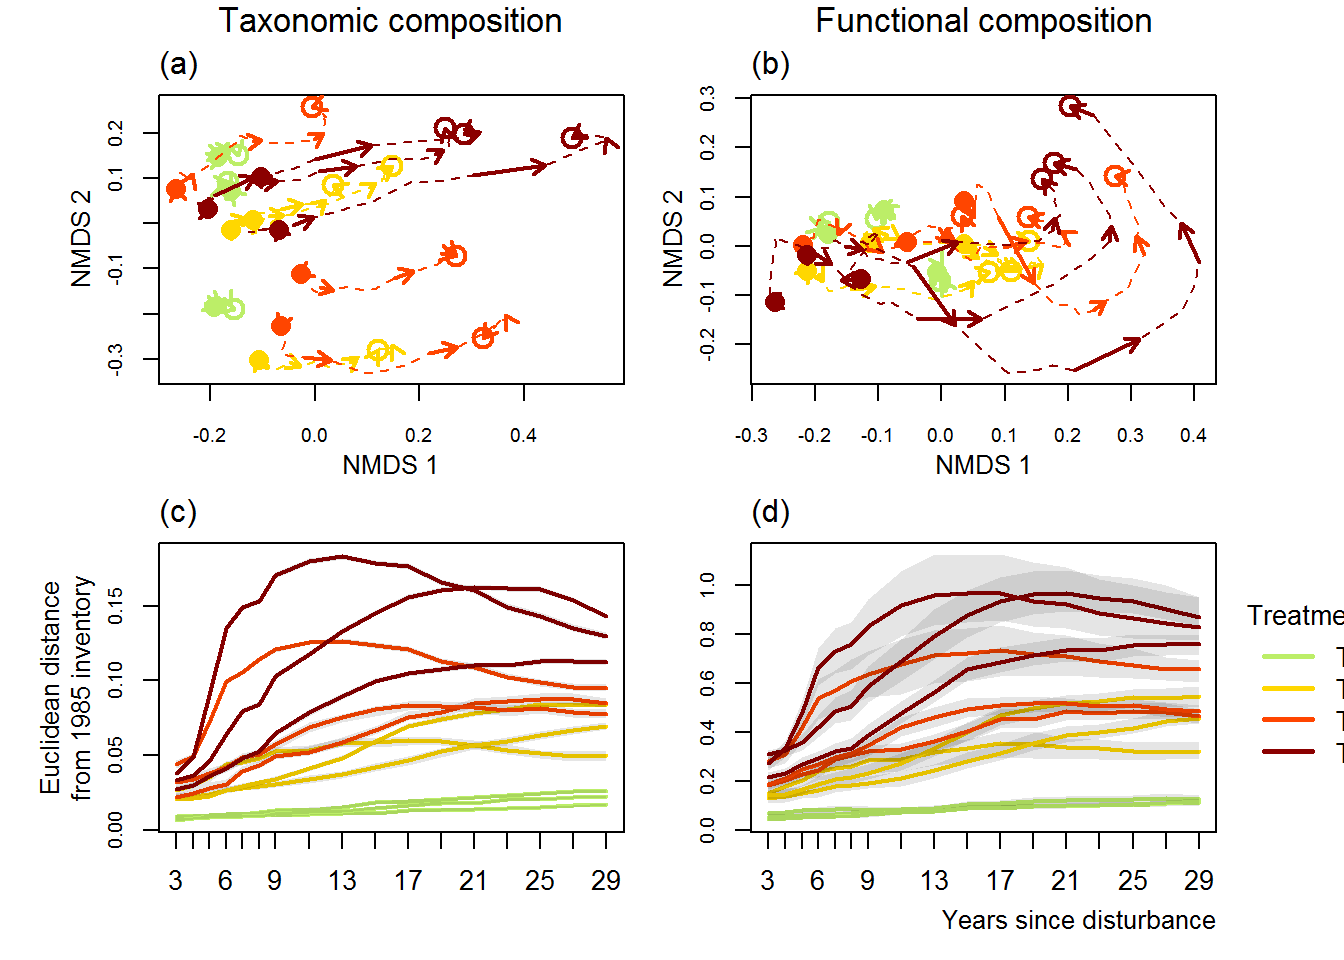
\includegraphics[width=1\linewidth]{WholePlotTrajectories_files/figure-latex/NMDSplans-1} 

}

\caption{Plot trajectories in terms of taxonomic composition (\textbf{(a)} and \textbf{(c)}), and functional composition (\textbf{(b)} and \textbf{(d)}) in a two-dimensional NMDS plane. Lower panels (\textbf{(c)} and \textbf{(d)}) represent the Euclidean distance to initial condition along the 30 sampled years. Shaded areas are the credibility intervals.}\label{fig:NMDSplans}
\end{figure*}

In control plots, Community Weighted Means (CWM) of functional traits
remained stable in time.\\
In disturbed plots, they mostly followed unimodal trajectories, either
stabilizing or returning towards their initial values, to the exception
of leaf chlorophyll content, which continued to increase 30 years after
disturbance for 4 out of 6 highly disturbed plots. Maximum height at
adult stage (\emph{Hmax}), leaf toughness, and wood specific gravity
(\emph{WSG}) decreased in time and then slightly increased, but remained
significantly lower than their initial value (Fig. \ref{fig:CWM}). Bark
thickness and specific leaf area (\emph{SLA}) both increased along time.
Bark thickness remained substantially high after 30 years, and
\emph{SLA} had almost recovered to its initial value. Whatever the
functional traits, the maximum difference to initial value was highly
correlated to the disturbance intensity. Positive correlations were
observed for leaf thickness, chlorophyll content, SLA and bark thickness
(\(\rho_{Spearman}^{Leaf thickness}=0.76\),
\(\rho_{Spearman}^{Chlorophyll content}=0.60\),
\(\rho_{Spearman}^{SLA}=0.93\),
\(\rho_{Spearman}^{Bark thickness}=0.71\)). Negative correlation was
observed for leaf toughness, WSG, and Hmax
(\(\rho_{Spearman}^{Leaf toughness}=-0.53\),
\(\rho_{Spearman}^{WSG}=-0.75\), \(\rho_{Spearman}^{Hmax}=-0.40\)) The
proportions of the three lightest seed mass classes increased in all
disturbed plots. After 30 years the proportion of lightest seed mass
class decreased while it stabilized for the two other lightest seed mass
classes (Supp. Mat. - Fig. S2).

\begin{figure*}

{\centering 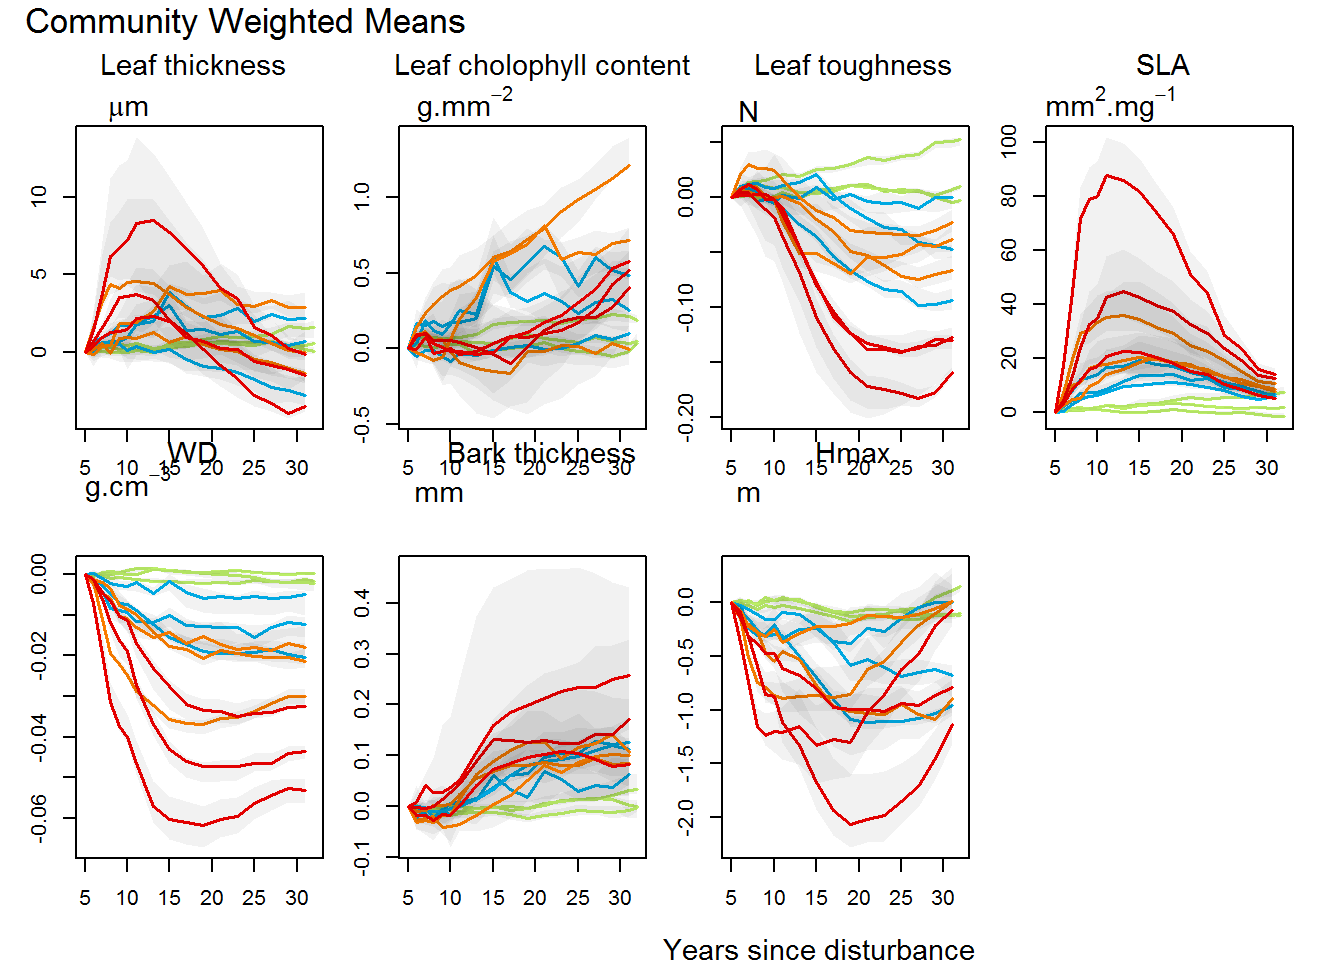
\includegraphics[width=1\linewidth]{WholePlotTrajectories_files/figure-latex/CWM-1} 

}

\caption{Trajectories of community weighted means over 30 years after disturbance of four leaf traits (leaf thickness, chlorophyll content, toughness, and specific area), two stem traits (wood specific gravity and bark thickness), and one life history trait (species maximum height at adult stage). }\label{fig:CWM}
\end{figure*}

\subsection{Community taxonomic and functional
diversity}\label{community-taxonomic-and-functional-diversity}

Taxonomic richness and evenness remained stable in control plots over
the 30 years of monitoring. In disturbed communities, after low
disturbance intensity the taxonomic richness increased, reaching a
maximum gain of 14 botanical genera. After intense disturbance the
taxonomic richness followed a more complex trajectory, decreasing for
ten years after disturbance before recovering to pre-disturbance values.
The maximum richness loss or gain after disturbance was positively
correlated with the disturbance intensity
(\(\rho_{Spearman}^{Richness}=0.50\)).

In all disturbed plots the evenness first increased until a maximum
reached after around 20 years. This maximum was positively correlated
with the disturbance intensity (\(\rho_{Spearman}^{Simpson}=0.77\)). The
evenness then stabilized except for two intensively-disturbed plots
(number 8 and 12) for which it kept increasing (Fig. \ref{fig:DivTaxo}).

\begin{figure*}

{\centering 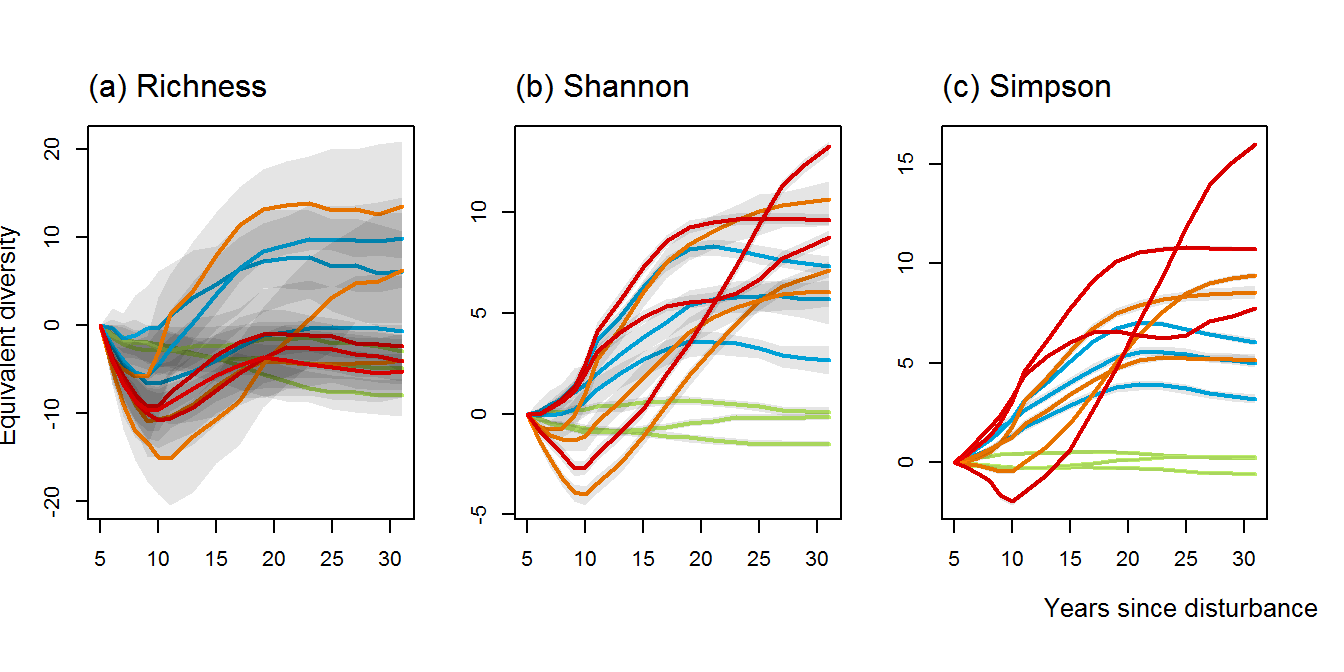
\includegraphics[width=1\linewidth]{WholePlotTrajectories_files/figure-latex/DivTaxo-1} 

}

\caption{Trajectories of community taxonomic richness \textbf{(a)}, Simpson diversity \textbf{(b)}, functional richness \textbf{(c)}, and Rao diversity \textbf{(d)}. Values correspond to the difference over 30 years of community diversity with the values of 1984 pre-disturbance inventories of reference. Shaded areas are the credibility intervals }\label{fig:DivTaxo}
\end{figure*}

Functional richness and evenness remained stable in control plots over
the 30 years of monitoring. In disturbed communities, both trajectories
depended on the disturbance intensity, with their maximum values in time
being positively correlated to \%AGB loss
\(\rho_{Spearman}^{Richness} = 0.76\) and\\
\(\rho_{Spearman}^{Rao} = 0.60\). For low disturbance intensity,
functional richness and evenness displayed a low but long-lasting
increase up to a maximum reached after 20-25 years. For high disturbance
intensity, they generally displayed a fast but short increase followed,
after 10 years, by a slow decrease towards the initial values.

The second-degree polynomial regressions between (i) the percentage AGB
loss, and (ii) the taxonomic and functional diversity showed various
shapes depending on the diversity indices and on the time since
disturbance (Fig. \ref{fig:IDHplot}). Regarding taxonomic diversity, the
relationship between disturbance intensity and diversity was more
markedly hump-shaped for richness than for evenness, and peaked at 20\%
of initial AGB loss. Regarding functional diversity, the relationship
was almost linear, and was similar between richness and evenness. All
the relationships between disturbance intensity and diversity were
stronger 20 or 30 years after disturbance than they were 10 years after
disturbance.

\begin{figure*}

{\centering 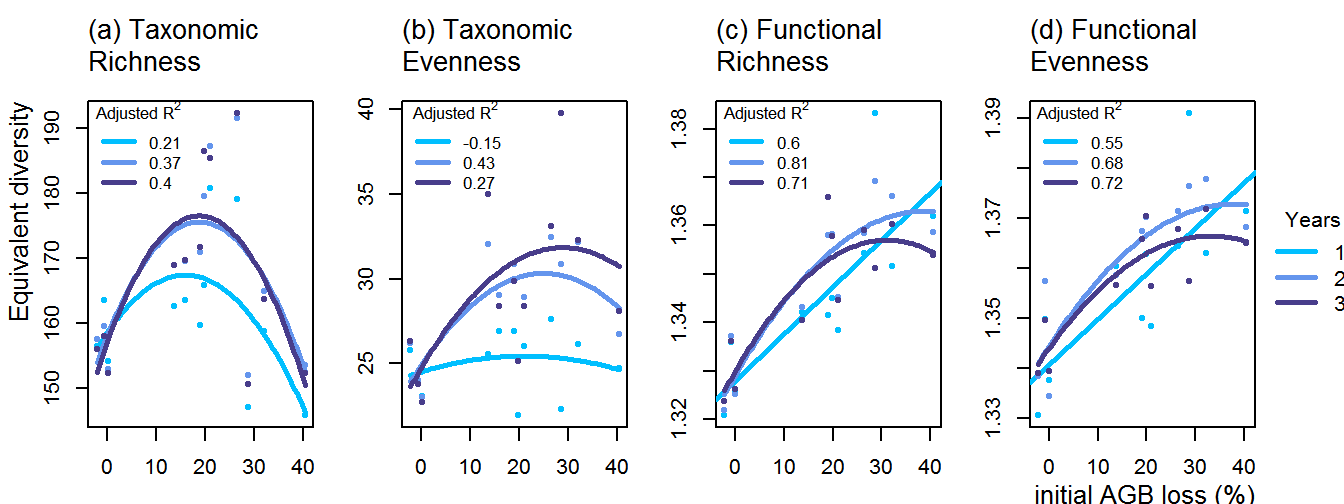
\includegraphics[width=1\linewidth]{WholePlotTrajectories_files/figure-latex/IDHplot-1} 

}

\caption{Relationship between the initial \%AGB loss and community taxonomic richness \textbf{(a)}, taxonomic evenness \textbf{(b)}, functional richness \textbf{(c)}, and functional evenness \textbf{(d)} at 10, 20, and 30 years after disturbance.}\label{fig:IDHplot}
\end{figure*}

\subsection{Functional redundancy}\label{functional-redundancy}

Control plots displayed stable functional redundancy over time. All
disturbed plots had lower functional redundancy than control plots and
followed similar hump-shaped trajectories (Fig. \ref{fig:RedFunRest}).
The maximum redundancy loss was positively correlated with the
disturbance intensity (\(\rho_{Spearman}=0.47\)) and the recovery
trajectory had not attained initial values for any disturbed communities
after 30 years.

\begin{figure}

{\centering 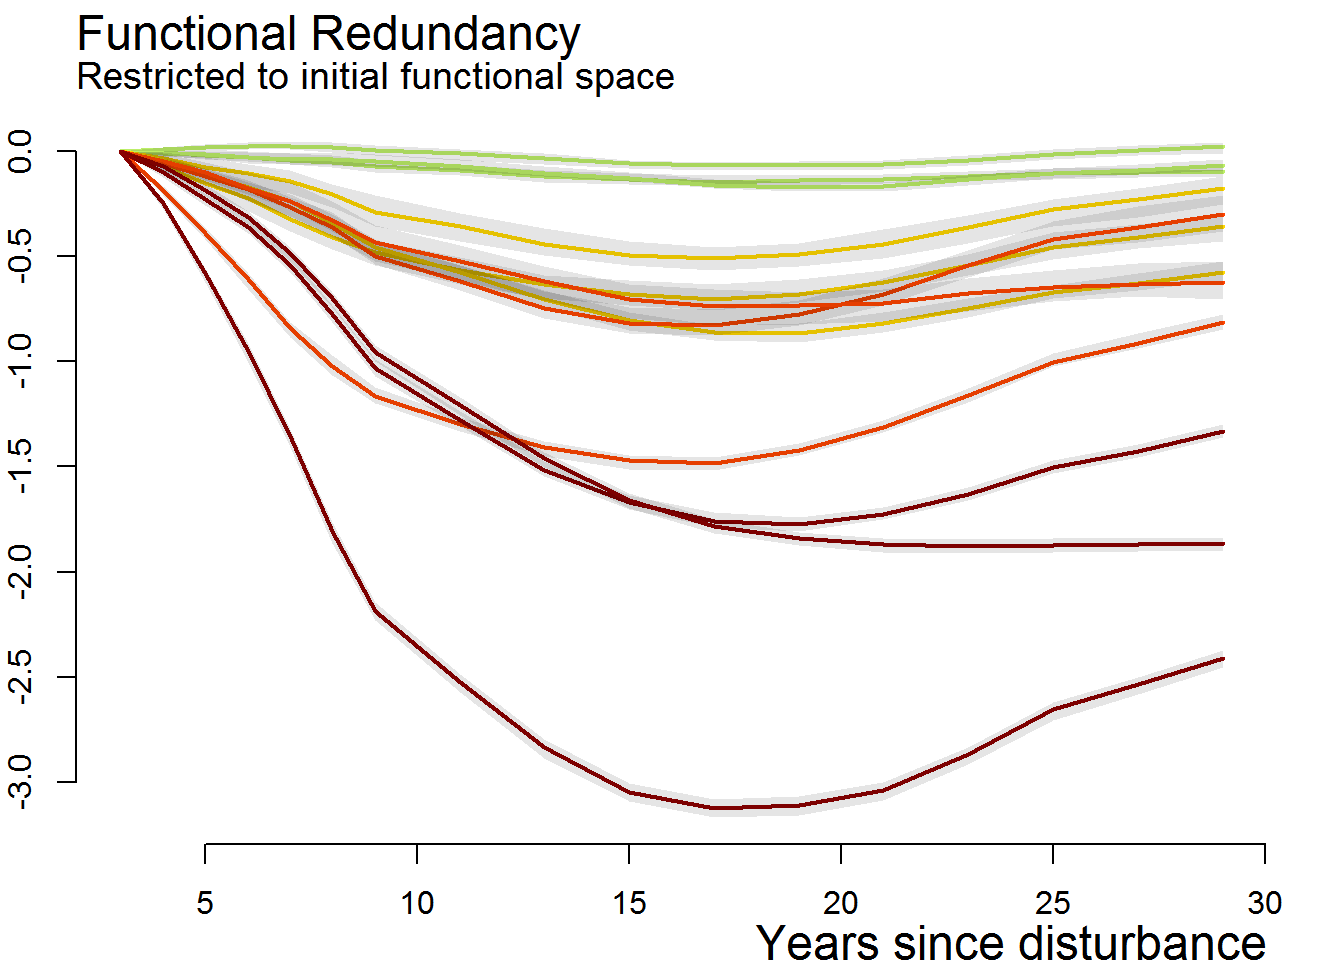
\includegraphics[width=1\linewidth]{WholePlotTrajectories_files/figure-latex/RedFunRest-1} 

}

\caption{Trajectories of the functional redundancy within the initial functional space over 30 years after disturbance. Shaded areas are the credibility intervals.}\label{fig:RedFunRest}
\end{figure}

\section{Discussion}\label{discussion}

Our analysis revealed the decoupling between functional and taxonomic
trajectories. While the initial differences in taxonomic composition
among plots were maintained, the functional composition trajectories
converged in the functional space. In terms of diversity, only the
taxonomic trajectories validated the IDH that explained humped-shaped
post-disturbance trajectories whith an amplitude depending on the
disturbance intensity. The decoupling between taxonomic and functional
response was explained by variations of community functional redundancy
that mitigated the functional impact of disturbance, and appeared as a
determinant of community recovery.

\subsection{Decoupled taxonomic and functional
trajectories}\label{decoupled-taxonomic-and-functional-trajectories}

Community taxonomic composition substantially differed before
disturbance, as materialized by their distinct location on the NMDS axis
2. These initial differences were maintained along the 30 years
following disturbance, with the disturbance leading a displacement on
the NMDS axis 1 only. Taxonomic composition changes were similar among
plots and may correspond to the recruitment of a group of pioneers, like
\emph{Cecropia spp.} or \emph{Miconia spp.}, common to all plots,
whatever their initial taxonomic differences and the intensity of
disturbance \citep{Denslow2000, Bongers2009}. Taxonomic trajectories
initiated a recovery towards the initial composition. This recovery,
although far from being achieved after 30 years, suggested the
resilience of community taxonomic composition and the maintenance of
initial composition differences \citep{Folke2006}. Such resilience
suggested that species not belonging to the pre-disturbance community
were rarely recruited in the long-term, probably because of species
dispersal limitation that is common among tropical species
\citep{Svenning2005}.

Community functional composition trajectories, in contrast, were similar
in the functional space \citep{Fukami2005}. The amplitude of the
compositional changes depended on the disturbance intensity. Functional
trajectories were probably driven by the recruitment of species
infrequent or absent before disturbance, and belonging to a pool of
species common to all plots. This common pool was composed of pioneers
with ``resource-acquisitive''" strategies displaying low leaf toughness,
wood specific gravity, maximum height, and high specific leaf area. The
recruitment of these pioneers drove a displacement to the right along
the first NMDS axis \citep{Westoby1998, Wright2004, Reich2014}.
Thereafter, the first recruited pioneers were progressively excluded by
long-lived, more competitive, and shade-tolerant species. The
recruitment of these late-successionals marked the recovery of the
initial functional composition with more ``resource-conservative''"
strategies . This recovery translated in the functional plane by a
displacement left along the first axis and upward along the second axis
(Fig. \ref{fig:NMDSplans}).

The decoupling between taxonomic and functional trajectories suggested
that simultaneous operation of trait-based assembly rules and
species-level priority effects shaped tree community assembly in Paracou
forest. Tree community assembly would then be both deterministic in the
functional space, and historically contingent in the taxonomic space.

\subsection{The scope of the intermediate disturbance
hypothesis}\label{the-scope-of-the-intermediate-disturbance-hypothesis}

Trajectories of taxonomic richness and evenness differed markedly below
and above an intensity threshold (Fig. \ref{fig:DivTaxo}). For low and
intermediate disturbance, both taxonomic richness and evenness increased
according to the disturbance intensity
\citep{Martin2015, Chaudhary2016}. This suggested that the recruitment
of pioneers, previously infrequent or absent, increased the taxonomic
richness \citep{Martin2015, Chaudhary2016}, and that trees surviving
after disturbance remained numerous enough to maintain the richness of
the pre-disturbance community \citep{Bongers2009}. The pioneers thus
recruited became abundant, which balanced the usual hyper-dominance of
tropical forests and increased the taxonomic evenness
\citep{Baraloto2012a}. Above the intensity threshold, like for treatment
3 (high intensity), the taxonomic richness did not exceed the initial
value in the first years following disturbance. No increase of the
taxonomic richness suggested that the richness of surviving trees was
lower than this of the pre-disturbance community, and that this
difference was not offset by the recruitment of pioneers. In the Guiana
shield, the pool of true pioneers specifically recruited after
disturbance is restricted to a few common genera (e.g. \emph{Cecropia
spp.}, \emph{Miconia spp.}, \emph{Tapirira spp.}) \citep{Guitet2018}.
Considering the different times after disturbance, there was always a
humped-shaped pattern linking the disturbance intensity with the
post-disturbance increase in taxonomic richness and evenness (Fig.
\ref{fig:IDHplot}). Both taxonomic richness and evenness were maximized
at an intermediate intensity, around 20-25\% of AGB lost.

Regarding community functional trajectories, however, no marked
differences were observed among post-disturbance trajectories (Fig.
\ref{fig:DivTaxo}). Whenever the disturbance intensity, there was first
an increase of both functional richness and evenness. Such increase
suggested the recruitment of pioneers that were functionally highly
different from the pre-disturbance community
\citep{Denslow1980, Molino2001}. The recruitment of pioneers hampered
the recruitment of other species in the first place. After 15 to 20
years, the first pioneer recruits declined and were replaced by species
functionally more similar to the pre-disturbance community, which
decreased the functional richness and evenness \citep{Walker2009}.

\subsection{The functional redundancy, key of community
resilience}\label{the-functional-redundancy-key-of-community-resilience}

The loss of species following disturbance decreased community functional
redundancy during the first 15 years. Progressively though, the
functional redundancy was restored through the replacement of the
species with ``resource-acquisitive''" strategies by more
late-successional species, functionally closer to the pre-disturbance
community. The replacement of pioneers by late-successionals followed
the lottery recruitment rules. This rules mean an easy recruitment of
the first species that becomes increasingly difficult, as the following
species are hampered by the emergence of interspecific competition
\citep{Busing2002}. The increasing competition among species explained
why the recovery trajectory slowed down 20 years after disturbance. The
recovery of the functional redundancy then relied upon the random
process of species recruitment, and was increasingly slow and difficult
to anticipate \citep{Elmqvist2003, Diaz2005}. This suggested a low
resilience of the functional redundancy with the random recovery of
infrequent species increasing the risks of losing keystone species, with
unexpected ecological consequences
\citep{Jones1994, Chazdon2003a, Diaz2005}. Infrequent species might
indeed have unique functional characteristics in the ecosystem, apart
from the ones considered here, in the ecosystem or be a key resource for
some of the fauna \citep{Schleuning2016}.

\section{Conclusion}\label{conclusion}

Post-disturbance trajectories of tree community composition and
diversity were driven by the recruitment of a determined pool of
pioneers, identical among local communities, and independent of the
disturbance intensity. The taxonomic composition trajectories maintained
the initial differences among communities, while the functional
trajectories were similar, and converged in the functional space towards
the recovery of the initial composition. The diversity trajectories were
contrasted as well. While the functional trajectories remained similar
whatever the disturbance intensity, taxonomic trajectories were markedly
different from a threshold of 20-25\% AGB lost that maximized the
taxonomic richness. The Intermediate Disturbance Hypothesis applied well
to taxonomic diversity, but not to functional diversity. The decoupling
between taxonomic and functional trajectories was mediated by the
variations in functional redundancy, as the loss of a species does not
necessarily entails the loss of its functional characteristics.
Community resilience, in terms of recovery of the pre-disturbance state,
was tangible but required several decades, and relied upon the random
lottery recruitment of rare species. Given the long-term impacts of
disturbance observed, we suggest that 30 years is not enough time for
tropical communities to recover, even after relatively low intensity
disturbance. Much of community response to disturbance rely on the
processes of species recruitment. A more refined understanding of the
post-disturbance trajectories would be gained by a closer analysis of
the recruitment process.

\section{Acknowledgement}\label{acknowledgement}

We are in debt with all Paracou station technicians and colleagues who
helped setting up the plots and collecting data over years. Without
their precious work, this study would have not been possible and they
may be warmly thanked here. Our work benefited from an ``Investissement
d'Avenir'' grant managed by the Agence Nationale de la Recherche (LABEX
CEBA, ref ANR-10-LBX-25). We thank Niklas Tysklind for the usefull help
with english proofing.

\section{Author's contributions}\label{authors-contributions}

AM, EM \& BH designed the study, developed the analysis framework, and
interpreted the results. AM wrote the manuscript with contributions by
EM \& BH. All authors gave final approval for publication.

\section{Data availability}\label{data-availability}

This article is based upon the dataset of the Paracou station, which is
part of the Guyafor permanent plot network in French Guiana
(Cirad-CNRS-ONF). The dataset is available upon request to the
scientific director (https://paracou.cirad.fr).

%----------------------------------------------------------------------------------------
%	REFERENCE LIST
%----------------------------------------------------------------------------------------

\bibliographystyle{mee}
\makeatletter
% The filename has .bib extension the must be eliminated
\filename@parse{references.bib}
% parse stores the file name in base. Extension starts at the first dot, so don't use dots in file names.
\bibliography{\filename@base}
\makeatother


%----------------------------------------------------------------------------------------

\end{document}
